\documentclass[1p]{elsarticle_modified}
%\bibliographystyle{elsarticle-num}

%\usepackage[colorlinks]{hyperref}
%\usepackage{abbrmath_seonhwa} %\Abb, \Ascr, \Acal ,\Abf, \Afrak
\usepackage{amsfonts}
\usepackage{amssymb}
\usepackage{amsmath}
\usepackage{amsthm}
\usepackage{scalefnt}
\usepackage{amsbsy}
\usepackage{kotex}
\usepackage{caption}
\usepackage{subfig}
\usepackage{color}
\usepackage{graphicx}
\usepackage{xcolor} %% white, black, red, green, blue, cyan, magenta, yellow
\usepackage{float}
\usepackage{setspace}
\usepackage{hyperref}

\usepackage{tikz}
\usetikzlibrary{arrows}

\usepackage{multirow}
\usepackage{array} % fixed length table
\usepackage{hhline}

%%%%%%%%%%%%%%%%%%%%%
\makeatletter
\renewcommand*\env@matrix[1][\arraystretch]{%
	\edef\arraystretch{#1}%
	\hskip -\arraycolsep
	\let\@ifnextchar\new@ifnextchar
	\array{*\c@MaxMatrixCols c}}
\makeatother %https://tex.stackexchange.com/questions/14071/how-can-i-increase-the-line-spacing-in-a-matrix
%%%%%%%%%%%%%%%

\usepackage[normalem]{ulem}

\newcommand{\msout}[1]{\ifmmode\text{\sout{\ensuremath{#1}}}\else\sout{#1}\fi}
%SOURCE: \msout is \stkout macro in https://tex.stackexchange.com/questions/20609/strikeout-in-math-mode

\newcommand{\cancel}[1]{
	\ifmmode
	{\color{red}\msout{#1}}
	\else
	{\color{red}\sout{#1}}
	\fi
}

\newcommand{\add}[1]{
	{\color{blue}\uwave{#1}}
}

\newcommand{\replace}[2]{
	\ifmmode
	{\color{red}\msout{#1}}{\color{blue}\uwave{#2}}
	\else
	{\color{red}\sout{#1}}{\color{blue}\uwave{#2}}
	\fi
}

\newcommand{\Sol}{\mathcal{S}} %segment
\newcommand{\D}{D} %diagram
\newcommand{\A}{\mathcal{A}} %arc


%%%%%%%%%%%%%%%%%%%%%%%%%%%%%5 test

\def\sl{\operatorname{\textup{SL}}(2,\Cbb)}
\def\psl{\operatorname{\textup{PSL}}(2,\Cbb)}
\def\quan{\mkern 1mu \triangleright \mkern 1mu}

\theoremstyle{definition}
\newtheorem{thm}{Theorem}[section]
\newtheorem{prop}[thm]{Proposition}
\newtheorem{lem}[thm]{Lemma}
\newtheorem{ques}[thm]{Question}
\newtheorem{cor}[thm]{Corollary}
\newtheorem{defn}[thm]{Definition}
\newtheorem{exam}[thm]{Example}
\newtheorem{rmk}[thm]{Remark}
\newtheorem{alg}[thm]{Algorithm}

\newcommand{\I}{\sqrt{-1}}
\begin{document}

%\begin{frontmatter}
%
%\title{Boundary parabolic representations of knots up to 8 crossings}
%
%%% Group authors per affiliation:
%\author{Yunhi Cho} 
%\address{Department of Mathematics, University of Seoul, Seoul, Korea}
%\ead{yhcho@uos.ac.kr}
%
%
%\author{Seonhwa Kim} %\fnref{s_kim}}
%\address{Center for Geometry and Physics, Institute for Basic Science, Pohang, 37673, Korea}
%\ead{ryeona17@ibs.re.kr}
%
%\author{Hyuk Kim}
%\address{Department of Mathematical Sciences, Seoul National University, Seoul 08826, Korea}
%\ead{hyukkim@snu.ac.kr}
%
%\author{Seokbeom Yoon}
%\address{Department of Mathematical Sciences, Seoul National University, Seoul, 08826,  Korea}
%\ead{sbyoon15@snu.ac.kr}
%
%\begin{abstract}
%We find all boundary parabolic representation of knots up to 8 crossings.
%
%\end{abstract}
%\begin{keyword}
%    \MSC[2010] 57M25 
%\end{keyword}
%
%\end{frontmatter}

%\linenumbers
%\tableofcontents
%
\newcommand\colored[1]{\textcolor{white}{\rule[-0.35ex]{0.8em}{1.4ex}}\kern-0.8em\color{red} #1}%
%\newcommand\colored[1]{\textcolor{white}{ #1}\kern-2.17ex	\textcolor{white}{ #1}\kern-1.81ex	\textcolor{white}{ #1}\kern-2.15ex\color{red}#1	}

{\Large $\underline{12a_{0125}~(K12a_{0125})}$}

\setlength{\tabcolsep}{10pt}
\renewcommand{\arraystretch}{1.6}
\vspace{1cm}\begin{tabular}{m{100pt}>{\centering\arraybackslash}m{274pt}}
\multirow{5}{120pt}{
	\centering
	\includegraphics[width=112pt]{../../../GIT/diagram.site/Diagrams/png/926_12a_0125.png}\\
\ \ \ A knot diagram\footnotemark}&
\allowdisplaybreaks
\textbf{Linearized knot diagam} \\
\cline{2-2}
 &
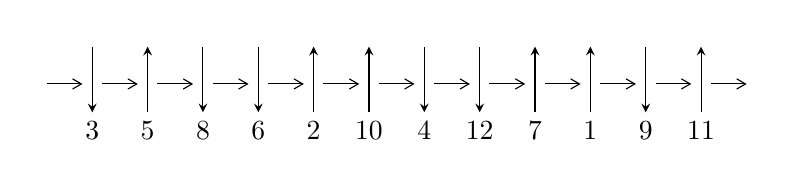
\begin{tikzpicture}[x=20pt, y=17pt]
	% nodes
	\node (C0) at (0, 0) {};
	\node (C1) at (1, 0) {};
	\node (C1U) at (1, +1) {};
	\node (C1D) at (1, -1) {3};

	\node (C2) at (2, 0) {};
	\node (C2U) at (2, +1) {};
	\node (C2D) at (2, -1) {5};

	\node (C3) at (3, 0) {};
	\node (C3U) at (3, +1) {};
	\node (C3D) at (3, -1) {8};

	\node (C4) at (4, 0) {};
	\node (C4U) at (4, +1) {};
	\node (C4D) at (4, -1) {6};

	\node (C5) at (5, 0) {};
	\node (C5U) at (5, +1) {};
	\node (C5D) at (5, -1) {2};

	\node (C6) at (6, 0) {};
	\node (C6U) at (6, +1) {};
	\node (C6D) at (6, -1) {10};

	\node (C7) at (7, 0) {};
	\node (C7U) at (7, +1) {};
	\node (C7D) at (7, -1) {4};

	\node (C8) at (8, 0) {};
	\node (C8U) at (8, +1) {};
	\node (C8D) at (8, -1) {12};

	\node (C9) at (9, 0) {};
	\node (C9U) at (9, +1) {};
	\node (C9D) at (9, -1) {7};

	\node (C10) at (10, 0) {};
	\node (C10U) at (10, +1) {};
	\node (C10D) at (10, -1) {1};

	\node (C11) at (11, 0) {};
	\node (C11U) at (11, +1) {};
	\node (C11D) at (11, -1) {9};

	\node (C12) at (12, 0) {};
	\node (C12U) at (12, +1) {};
	\node (C12D) at (12, -1) {11};
	\node (C13) at (13, 0) {};

	% arrows
	\draw[->,>={angle 60}]
	(C0) edge (C1) (C1) edge (C2) (C2) edge (C3) (C3) edge (C4) (C4) edge (C5) (C5) edge (C6) (C6) edge (C7) (C7) edge (C8) (C8) edge (C9) (C9) edge (C10) (C10) edge (C11) (C11) edge (C12) (C12) edge (C13) ;	\draw[->,>=stealth]
	(C1U) edge (C1D) (C2D) edge (C2U) (C3U) edge (C3D) (C4U) edge (C4D) (C5D) edge (C5U) (C6D) edge (C6U) (C7U) edge (C7D) (C8U) edge (C8D) (C9D) edge (C9U) (C10D) edge (C10U) (C11U) edge (C11D) (C12D) edge (C12U) ;
	\end{tikzpicture} \\
\hhline{~~} \\& 
\textbf{Solving Sequence} \\ \cline{2-2} 
 &
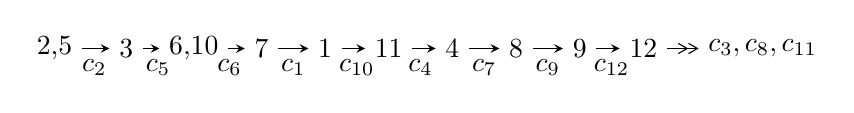
\begin{tikzpicture}[x=23pt, y=7pt]
	% node
	\node (A0) at (-1/8, 0) {2,5};
	\node (A1) at (1, 0) {3};
	\node (A2) at (33/16, 0) {6,10};
	\node (A3) at (25/8, 0) {7};
	\node (A4) at (33/8, 0) {1};
	\node (A5) at (41/8, 0) {11};
	\node (A6) at (49/8, 0) {4};
	\node (A7) at (57/8, 0) {8};
	\node (A8) at (65/8, 0) {9};
	\node (A9) at (73/8, 0) {12};
	\node (C1) at (1/2, -1) {$c_{2}$};
	\node (C2) at (3/2, -1) {$c_{5}$};
	\node (C3) at (21/8, -1) {$c_{6}$};
	\node (C4) at (29/8, -1) {$c_{1}$};
	\node (C5) at (37/8, -1) {$c_{10}$};
	\node (C6) at (45/8, -1) {$c_{4}$};
	\node (C7) at (53/8, -1) {$c_{7}$};
	\node (C8) at (61/8, -1) {$c_{9}$};
	\node (C9) at (69/8, -1) {$c_{12}$};
	\node (A10) at (11, 0) {$c_{3},c_{8},c_{11}$};

	% edge
	\draw[->,>=stealth]	
	(A0) edge (A1) (A1) edge (A2) (A2) edge (A3) (A3) edge (A4) (A4) edge (A5) (A5) edge (A6) (A6) edge (A7) (A7) edge (A8) (A8) edge (A9) ;
	\draw[->>,>={angle 60}]	
	(A9) edge (A10);
\end{tikzpicture} \\ 

\end{tabular} \\

\footnotetext{
The image of knot diagram is generated by the software ``\textbf{Draw programme}" developed by Andrew Bartholomew(\url{http://www.layer8.co.uk/maths/draw/index.htm\#Running-draw}), where we modified some parts for our purpose(\url{https://github.com/CATsTAILs/LinksPainter}).
}\phantom \\ \newline 
\centering \textbf{Ideals for irreducible components\footnotemark of $X_{\text{par}}$} 
 
\begin{align*}
I^u_{1}&=\langle 
-1.45958\times10^{63} u^{105}+1.24016\times10^{64} u^{104}+\cdots+1.23680\times10^{62} b+3.05806\times10^{63},\\
\phantom{I^u_{1}}&\phantom{= \langle  }1.13273\times10^{63} u^{105}-4.16667\times10^{63} u^{104}+\cdots+1.23680\times10^{62} a+4.77555\times10^{62},\;u^{106}-7 u^{105}+\cdots+11 u+1\rangle \\
I^u_{2}&=\langle 
b- a,\;- u^3 a+u^2 a+2 u^3+a^2-2 u^2- a+u+2,\;u^4- u^3+u^2+1\rangle \\
I^u_{3}&=\langle 
- a^2-2 a u+b- a+u+1,\;a^4+3 a^3 u-4 a^2 u-4 a^2+3 a+2 u,\;u^2+u+1\rangle \\
\\
\end{align*}
\raggedright * 3 irreducible components of $\dim_{\mathbb{C}}=0$, with total 122 representations.\\
\footnotetext{All coefficients of polynomials are rational numbers. But the coefficients are sometimes approximated in decimal forms when there is not enough margin.}
\newpage
\renewcommand{\arraystretch}{1}
\centering \section*{I. $I^u_{1}= \langle -1.46\times10^{63} u^{105}+1.24\times10^{64} u^{104}+\cdots+1.24\times10^{62} b+3.06\times10^{63},\;1.13\times10^{63} u^{105}-4.17\times10^{63} u^{104}+\cdots+1.24\times10^{62} a+4.78\times10^{62},\;u^{106}-7 u^{105}+\cdots+11 u+1 \rangle$}
\flushleft \textbf{(i) Arc colorings}\\
\begin{tabular}{m{7pt} m{180pt} m{7pt} m{180pt} }
\flushright $a_{2}=$&$\begin{pmatrix}1\\0\end{pmatrix}$ \\
\flushright $a_{5}=$&$\begin{pmatrix}0\\u\end{pmatrix}$ \\
\flushright $a_{3}=$&$\begin{pmatrix}1\\- u^2\end{pmatrix}$ \\
\flushright $a_{6}=$&$\begin{pmatrix}u\\u\end{pmatrix}$ \\
\flushright $a_{10}=$&$\begin{pmatrix}-9.15857 u^{105}+33.6892 u^{104}+\cdots-78.0000 u-3.86123\\11.8013 u^{105}-100.272 u^{104}+\cdots-296.223 u-24.7257\end{pmatrix}$ \\
\flushright $a_{7}=$&$\begin{pmatrix}16.6772 u^{105}-80.6901 u^{104}+\cdots+74.7375 u+5.64569\\-11.0849 u^{105}+100.425 u^{104}+\cdots+353.574 u+29.7886\end{pmatrix}$ \\
\flushright $a_{1}=$&$\begin{pmatrix}u^2+1\\- u^4\end{pmatrix}$ \\
\flushright $a_{11}=$&$\begin{pmatrix}-12.1515 u^{105}+46.3650 u^{104}+\cdots-82.9557 u-3.61751\\15.2241 u^{105}-129.122 u^{104}+\cdots-378.079 u-31.6912\end{pmatrix}$ \\
\flushright $a_{4}=$&$\begin{pmatrix}u^3\\u^3+u\end{pmatrix}$ \\
\flushright $a_{8}=$&$\begin{pmatrix}16.8295 u^{105}-91.5401 u^{104}+\cdots+41.0065 u+2.64419\\-10.2180 u^{105}+87.5744 u^{104}+\cdots+321.926 u+27.0475\end{pmatrix}$ \\
\flushright $a_{9}=$&$\begin{pmatrix}-15.3972 u^{105}+68.9700 u^{104}+\cdots-43.5872 u-1.83722\\13.1838 u^{105}-116.844 u^{104}+\cdots-377.008 u-31.4529\end{pmatrix}$ \\
\flushright $a_{12}=$&$\begin{pmatrix}3.05675 u^{105}-23.6825 u^{104}+\cdots+23.3656 u-0.183695\\-0.478044 u^{105}+1.52825 u^{104}+\cdots+34.1625 u+2.46930\end{pmatrix}$\\&\end{tabular}
\flushleft \textbf{(ii) Obstruction class $= -1$}\\~\\
\flushleft \textbf{(iii) Cusp Shapes $= -23.7616 u^{105}+179.119 u^{104}+\cdots+290.283 u+26.9682$}\\~\\
\newpage\renewcommand{\arraystretch}{1}
\flushleft \textbf{(iv) u-Polynomials at the component}\newline \\
\begin{tabular}{m{50pt}|m{274pt}}
Crossings & \hspace{64pt}u-Polynomials at each crossing \\
\hline $$\begin{aligned}c_{1},c_{4}\end{aligned}$$&$\begin{aligned}
&u^{106}+35 u^{105}+\cdots+9 u+1
\end{aligned}$\\
\hline $$\begin{aligned}c_{2},c_{5}\end{aligned}$$&$\begin{aligned}
&u^{106}+7 u^{105}+\cdots-11 u+1
\end{aligned}$\\
\hline $$\begin{aligned}c_{3},c_{7}\end{aligned}$$&$\begin{aligned}
&u^{106}-3 u^{105}+\cdots-1152 u+256
\end{aligned}$\\
\hline $$\begin{aligned}c_{6},c_{9}\end{aligned}$$&$\begin{aligned}
&u^{106}+3 u^{105}+\cdots+1152 u+256
\end{aligned}$\\
\hline $$\begin{aligned}c_{8},c_{11}\end{aligned}$$&$\begin{aligned}
&u^{106}-7 u^{105}+\cdots+11 u+1
\end{aligned}$\\
\hline $$\begin{aligned}c_{10},c_{12}\end{aligned}$$&$\begin{aligned}
&u^{106}-35 u^{105}+\cdots-9 u+1
\end{aligned}$\\
\hline
\end{tabular}\\~\\
\newpage\renewcommand{\arraystretch}{1}
\flushleft \textbf{(v) Riley Polynomials at the component}\newline \\
\begin{tabular}{m{50pt}|m{274pt}}
Crossings & \hspace{64pt}Riley Polynomials at each crossing \\
\hline $$\begin{aligned}c_{1},c_{4},c_{10}\\c_{12}\end{aligned}$$&$\begin{aligned}
&y^{106}+79 y^{105}+\cdots+1045 y+1
\end{aligned}$\\
\hline $$\begin{aligned}c_{2},c_{5},c_{8}\\c_{11}\end{aligned}$$&$\begin{aligned}
&y^{106}+35 y^{105}+\cdots+9 y+1
\end{aligned}$\\
\hline $$\begin{aligned}c_{3},c_{6},c_{7}\\c_{9}\end{aligned}$$&$\begin{aligned}
&y^{106}+55 y^{105}+\cdots+1654784 y+65536
\end{aligned}$\\
\hline
\end{tabular}\\~\\
\newpage\flushleft \textbf{(vi) Complex Volumes and Cusp Shapes}
$$\begin{array}{c|c|c}  
\text{Solutions to }I^u_{1}& \I (\text{vol} + \sqrt{-1}CS) & \text{Cusp shape}\\
 \hline 
\begin{aligned}
u &= \phantom{-}0.183013 + 0.981284 I \\
a &= -0.250624 + 1.170010 I \\
b &= \phantom{-}1.19910 + 1.07703 I\end{aligned}
 & -8.23499 + 5.48524 I & \phantom{-0.000000 } 0 \\ \hline\begin{aligned}
u &= \phantom{-}0.183013 - 0.981284 I \\
a &= -0.250624 - 1.170010 I \\
b &= \phantom{-}1.19910 - 1.07703 I\end{aligned}
 & -8.23499 - 5.48524 I & \phantom{-0.000000 } 0 \\ \hline\begin{aligned}
u &= -0.608368 + 0.790031 I \\
a &= -1.71520 + 2.08278 I \\
b &= -2.34512 + 1.92007 I\end{aligned}
 & \phantom{-}0.476825 + 0.520416 I & \phantom{-0.000000 } 0 \\ \hline\begin{aligned}
u &= -0.608368 - 0.790031 I \\
a &= -1.71520 - 2.08278 I \\
b &= -2.34512 - 1.92007 I\end{aligned}
 & \phantom{-}0.476825 - 0.520416 I & \phantom{-0.000000 } 0 \\ \hline\begin{aligned}
u &= -0.070703 + 0.979774 I \\
a &= \phantom{-}0.473670 + 1.255400 I \\
b &= \phantom{-}0.490461 + 0.187755 I\end{aligned}
 & -3.20551 + 0.41176 I & \phantom{-0.000000 } 0 \\ \hline\begin{aligned}
u &= -0.070703 - 0.979774 I \\
a &= \phantom{-}0.473670 - 1.255400 I \\
b &= \phantom{-}0.490461 - 0.187755 I\end{aligned}
 & -3.20551 - 0.41176 I & \phantom{-0.000000 } 0 \\ \hline\begin{aligned}
u &= -0.082433 + 1.016070 I \\
a &= -0.536516 - 0.233091 I \\
b &= -1.61438 - 0.31423 I\end{aligned}
 & -3.79720 - 2.42088 I & \phantom{-0.000000 } 0 \\ \hline\begin{aligned}
u &= -0.082433 - 1.016070 I \\
a &= -0.536516 + 0.233091 I \\
b &= -1.61438 + 0.31423 I\end{aligned}
 & -3.79720 + 2.42088 I & \phantom{-0.000000 } 0 \\ \hline\begin{aligned}
u &= \phantom{-}0.139173 + 1.012920 I \\
a &= \phantom{-}0.233853 - 0.977567 I \\
b &= -1.15979 - 0.93662 I\end{aligned}
 & -8.71380 - 0.62719 I & \phantom{-0.000000 } 0 \\ \hline\begin{aligned}
u &= \phantom{-}0.139173 - 1.012920 I \\
a &= \phantom{-}0.233853 + 0.977567 I \\
b &= -1.15979 + 0.93662 I\end{aligned}
 & -8.71380 + 0.62719 I & \phantom{-0.000000 } 0\\
 \hline 
 \end{array}$$\newpage$$\begin{array}{c|c|c}  
\text{Solutions to }I^u_{1}& \I (\text{vol} + \sqrt{-1}CS) & \text{Cusp shape}\\
 \hline 
\begin{aligned}
u &= -0.121668 + 1.027370 I \\
a &= -0.262202 - 1.241630 I \\
b &= -0.392812 - 0.212170 I\end{aligned}
 & -2.89214 - 5.06693 I & \phantom{-0.000000 } 0 \\ \hline\begin{aligned}
u &= -0.121668 - 1.027370 I \\
a &= -0.262202 + 1.241630 I \\
b &= -0.392812 + 0.212170 I\end{aligned}
 & -2.89214 + 5.06693 I & \phantom{-0.000000 } 0 \\ \hline\begin{aligned}
u &= \phantom{-}0.767026 + 0.703266 I \\
a &= \phantom{-}1.02342 + 1.09468 I \\
b &= \phantom{-}0.650088 - 0.104330 I\end{aligned}
 & \phantom{-}1.97848 - 2.25070 I & \phantom{-0.000000 } 0 \\ \hline\begin{aligned}
u &= \phantom{-}0.767026 - 0.703266 I \\
a &= \phantom{-}1.02342 - 1.09468 I \\
b &= \phantom{-}0.650088 + 0.104330 I\end{aligned}
 & \phantom{-}1.97848 + 2.25070 I & \phantom{-0.000000 } 0 \\ \hline\begin{aligned}
u &= -0.491542 + 0.815968 I \\
a &= \phantom{-}2.89723 - 2.04811 I \\
b &= \phantom{-}3.28360 - 1.89164 I\end{aligned}
 & \phantom{-0.000000 } -3.72687 I & \phantom{-0.000000 } 0 \\ \hline\begin{aligned}
u &= -0.491542 - 0.815968 I \\
a &= \phantom{-}2.89723 + 2.04811 I \\
b &= \phantom{-}3.28360 + 1.89164 I\end{aligned}
 & \phantom{-0.000000 -}3.72687 I & \phantom{-0.000000 } 0 \\ \hline\begin{aligned}
u &= \phantom{-}0.757210 + 0.725465 I \\
a &= \phantom{-}0.44531 + 1.47879 I \\
b &= \phantom{-}1.59591 + 1.06021 I\end{aligned}
 & \phantom{-}2.34132 + 0.87923 I & \phantom{-0.000000 } 0 \\ \hline\begin{aligned}
u &= \phantom{-}0.757210 - 0.725465 I \\
a &= \phantom{-}0.44531 - 1.47879 I \\
b &= \phantom{-}1.59591 - 1.06021 I\end{aligned}
 & \phantom{-}2.34132 - 0.87923 I & \phantom{-0.000000 } 0 \\ \hline\begin{aligned}
u &= \phantom{-}0.606407 + 0.862300 I \\
a &= \phantom{-}0.849818 - 0.206074 I \\
b &= -0.382310 - 1.247890 I\end{aligned}
 & -6.30345 - 0.88841 I & \phantom{-0.000000 } 0 \\ \hline\begin{aligned}
u &= \phantom{-}0.606407 - 0.862300 I \\
a &= \phantom{-}0.849818 + 0.206074 I \\
b &= -0.382310 + 1.247890 I\end{aligned}
 & -6.30345 + 0.88841 I & \phantom{-0.000000 } 0\\
 \hline 
 \end{array}$$\newpage$$\begin{array}{c|c|c}  
\text{Solutions to }I^u_{1}& \I (\text{vol} + \sqrt{-1}CS) & \text{Cusp shape}\\
 \hline 
\begin{aligned}
u &= \phantom{-}0.797191 + 0.698686 I \\
a &= -0.39788 - 1.50231 I \\
b &= -1.58826 - 1.20743 I\end{aligned}
 & \phantom{-}3.31076 - 4.88109 I & \phantom{-0.000000 } 0 \\ \hline\begin{aligned}
u &= \phantom{-}0.797191 - 0.698686 I \\
a &= -0.39788 + 1.50231 I \\
b &= -1.58826 + 1.20743 I\end{aligned}
 & \phantom{-}3.31076 + 4.88109 I & \phantom{-0.000000 } 0 \\ \hline\begin{aligned}
u &= -0.814211 + 0.692591 I \\
a &= \phantom{-}1.75987 - 0.39778 I \\
b &= \phantom{-}1.38167 + 0.58692 I\end{aligned}
 & -2.34132 - 0.87923 I & \phantom{-0.000000 } 0 \\ \hline\begin{aligned}
u &= -0.814211 - 0.692591 I \\
a &= \phantom{-}1.75987 + 0.39778 I \\
b &= \phantom{-}1.38167 - 0.58692 I\end{aligned}
 & -2.34132 + 0.87923 I & \phantom{-0.000000 } 0 \\ \hline\begin{aligned}
u &= \phantom{-}0.866786 + 0.634717 I \\
a &= \phantom{-}1.46524 + 1.07764 I \\
b &= \phantom{-}1.341270 - 0.241167 I\end{aligned}
 & \phantom{-0.000000 } -5.87854 I & \phantom{-0.000000 } 0 \\ \hline\begin{aligned}
u &= \phantom{-}0.866786 - 0.634717 I \\
a &= \phantom{-}1.46524 - 1.07764 I \\
b &= \phantom{-}1.341270 + 0.241167 I\end{aligned}
 & \phantom{-0.000000 -}5.87854 I & \phantom{-0.000000 } 0 \\ \hline\begin{aligned}
u &= -0.200048 + 1.057240 I \\
a &= \phantom{-}0.893176 - 0.486577 I \\
b &= \phantom{-}1.83864 - 0.23783 I\end{aligned}
 & \phantom{-0.000000 } -5.27517 I & \phantom{-0.000000 } 0 \\ \hline\begin{aligned}
u &= -0.200048 - 1.057240 I \\
a &= \phantom{-}0.893176 + 0.486577 I \\
b &= \phantom{-}1.83864 + 0.23783 I\end{aligned}
 & \phantom{-0.000000 -}5.27517 I & \phantom{-0.000000 } 0 \\ \hline\begin{aligned}
u &= -0.361209 + 1.017340 I \\
a &= -0.059410 - 0.516497 I \\
b &= -0.439695 + 0.151597 I\end{aligned}
 & \phantom{-}0.93508 - 1.21751 I & \phantom{-0.000000 } 0 \\ \hline\begin{aligned}
u &= -0.361209 - 1.017340 I \\
a &= -0.059410 + 0.516497 I \\
b &= -0.439695 - 0.151597 I\end{aligned}
 & \phantom{-}0.93508 + 1.21751 I & \phantom{-0.000000 } 0\\
 \hline 
 \end{array}$$\newpage$$\begin{array}{c|c|c}  
\text{Solutions to }I^u_{1}& \I (\text{vol} + \sqrt{-1}CS) & \text{Cusp shape}\\
 \hline 
\begin{aligned}
u &= \phantom{-}0.609367 + 0.892037 I \\
a &= -0.672343 + 0.456946 I \\
b &= \phantom{-}0.63191 + 1.33120 I\end{aligned}
 & -6.40447 + 5.65814 I & \phantom{-0.000000 } 0 \\ \hline\begin{aligned}
u &= \phantom{-}0.609367 - 0.892037 I \\
a &= -0.672343 - 0.456946 I \\
b &= \phantom{-}0.63191 - 1.33120 I\end{aligned}
 & -6.40447 - 5.65814 I & \phantom{-0.000000 } 0 \\ \hline\begin{aligned}
u &= \phantom{-}0.770716 + 0.767655 I \\
a &= -0.70064 - 1.22855 I \\
b &= -0.280019 - 0.215340 I\end{aligned}
 & \phantom{-}4.52079 + 2.63581 I & \phantom{-0.000000 } 0 \\ \hline\begin{aligned}
u &= \phantom{-}0.770716 - 0.767655 I \\
a &= -0.70064 + 1.22855 I \\
b &= -0.280019 + 0.215340 I\end{aligned}
 & \phantom{-}4.52079 - 2.63581 I & \phantom{-0.000000 } 0 \\ \hline\begin{aligned}
u &= -0.566270 + 0.934854 I \\
a &= \phantom{-}1.87881 - 1.90621 I \\
b &= \phantom{-}2.08787 - 1.30438 I\end{aligned}
 & -0.476825 - 0.520416 I & \phantom{-0.000000 } 0 \\ \hline\begin{aligned}
u &= -0.566270 - 0.934854 I \\
a &= \phantom{-}1.87881 + 1.90621 I \\
b &= \phantom{-}2.08787 + 1.30438 I\end{aligned}
 & -0.476825 + 0.520416 I & \phantom{-0.000000 } 0 \\ \hline\begin{aligned}
u &= -0.726604 + 0.816538 I \\
a &= -1.86538 + 1.02911 I \\
b &= -1.72394 + 0.15846 I\end{aligned}
 & \phantom{-}3.20551 - 0.41176 I & \phantom{-0.000000 } 0 \\ \hline\begin{aligned}
u &= -0.726604 - 0.816538 I \\
a &= -1.86538 - 1.02911 I \\
b &= -1.72394 - 0.15846 I\end{aligned}
 & \phantom{-}3.20551 + 0.41176 I & \phantom{-0.000000 } 0 \\ \hline\begin{aligned}
u &= \phantom{-}0.842877 + 0.705822 I \\
a &= -1.26558 - 1.34601 I \\
b &= -1.085060 - 0.187678 I\end{aligned}
 & \phantom{-}6.94581 - 5.02785 I & \phantom{-0.000000 } 0 \\ \hline\begin{aligned}
u &= \phantom{-}0.842877 - 0.705822 I \\
a &= -1.26558 + 1.34601 I \\
b &= -1.085060 + 0.187678 I\end{aligned}
 & \phantom{-}6.94581 + 5.02785 I & \phantom{-0.000000 } 0\\
 \hline 
 \end{array}$$\newpage$$\begin{array}{c|c|c}  
\text{Solutions to }I^u_{1}& \I (\text{vol} + \sqrt{-1}CS) & \text{Cusp shape}\\
 \hline 
\begin{aligned}
u &= \phantom{-}0.892716 + 0.645846 I \\
a &= -1.56857 - 1.13159 I \\
b &= -1.49793 + 0.16723 I\end{aligned}
 & \phantom{-}1.28626 - 11.79330 I & \phantom{-0.000000 } 0 \\ \hline\begin{aligned}
u &= \phantom{-}0.892716 - 0.645846 I \\
a &= -1.56857 + 1.13159 I \\
b &= -1.49793 - 0.16723 I\end{aligned}
 & \phantom{-}1.28626 + 11.79330 I & \phantom{-0.000000 } 0 \\ \hline\begin{aligned}
u &= -0.831655 + 0.735688 I \\
a &= -1.94362 + 0.45302 I \\
b &= -1.62921 - 0.57066 I\end{aligned}
 & -1.56866 + 4.68963 I & \phantom{-0.000000 } 0 \\ \hline\begin{aligned}
u &= -0.831655 - 0.735688 I \\
a &= -1.94362 - 0.45302 I \\
b &= -1.62921 + 0.57066 I\end{aligned}
 & -1.56866 - 4.68963 I & \phantom{-0.000000 } 0 \\ \hline\begin{aligned}
u &= -0.846903 + 0.235789 I \\
a &= -0.406411 + 0.154856 I \\
b &= \phantom{-}0.522749 - 0.873838 I\end{aligned}
 & -1.10077 - 7.84499 I & \phantom{-0.000000 } 0 \\ \hline\begin{aligned}
u &= -0.846903 - 0.235789 I \\
a &= -0.406411 - 0.154856 I \\
b &= \phantom{-}0.522749 + 0.873838 I\end{aligned}
 & -1.10077 + 7.84499 I & \phantom{-0.000000 } 0 \\ \hline\begin{aligned}
u &= -0.499442 + 0.720382 I \\
a &= \phantom{-}0.695312 - 0.877601 I \\
b &= \phantom{-}0.396527 - 0.460682 I\end{aligned}
 & \phantom{-}0.00288 - 1.41429 I & \phantom{-0.000000 } 0 \\ \hline\begin{aligned}
u &= -0.499442 - 0.720382 I \\
a &= \phantom{-}0.695312 + 0.877601 I \\
b &= \phantom{-}0.396527 + 0.460682 I\end{aligned}
 & \phantom{-}0.00288 + 1.41429 I & \phantom{-0.000000 } 0 \\ \hline\begin{aligned}
u &= -0.599521 + 0.957553 I \\
a &= \phantom{-}0.771353 - 1.121240 I \\
b &= \phantom{-}1.47129 - 1.34418 I\end{aligned}
 & -0.82280 - 3.12789 I & \phantom{-0.000000 } 0 \\ \hline\begin{aligned}
u &= -0.599521 - 0.957553 I \\
a &= \phantom{-}0.771353 + 1.121240 I \\
b &= \phantom{-}1.47129 + 1.34418 I\end{aligned}
 & -0.82280 + 3.12789 I & \phantom{-0.000000 } 0\\
 \hline 
 \end{array}$$\newpage$$\begin{array}{c|c|c}  
\text{Solutions to }I^u_{1}& \I (\text{vol} + \sqrt{-1}CS) & \text{Cusp shape}\\
 \hline 
\begin{aligned}
u &= -0.637724 + 0.932906 I \\
a &= -1.94663 + 1.67788 I \\
b &= -2.08360 + 0.92011 I\end{aligned}
 & \phantom{-0.000000 } -5.43693 I & \phantom{-0.000000 } 0 \\ \hline\begin{aligned}
u &= -0.637724 - 0.932906 I \\
a &= -1.94663 - 1.67788 I \\
b &= -2.08360 - 0.92011 I\end{aligned}
 & \phantom{-0.000000 -}5.43693 I & \phantom{-0.000000 } 0 \\ \hline\begin{aligned}
u &= -0.066695 + 0.862588 I \\
a &= \phantom{-}0.915878 + 1.066430 I \\
b &= \phantom{-}1.90466 + 0.87933 I\end{aligned}
 & -0.93508 + 1.21751 I & \phantom{-0.000000 } 0 \\ \hline\begin{aligned}
u &= -0.066695 - 0.862588 I \\
a &= \phantom{-}0.915878 - 1.066430 I \\
b &= \phantom{-}1.90466 - 0.87933 I\end{aligned}
 & -0.93508 - 1.21751 I & \phantom{-0.000000 } 0 \\ \hline\begin{aligned}
u &= -0.814464 + 0.288678 I \\
a &= \phantom{-}0.605911 - 0.175846 I \\
b &= -0.286730 + 0.819490 I\end{aligned}
 & -1.97848 - 2.25070 I & \phantom{-0.000000 } 0 \\ \hline\begin{aligned}
u &= -0.814464 - 0.288678 I \\
a &= \phantom{-}0.605911 + 0.175846 I \\
b &= -0.286730 - 0.819490 I\end{aligned}
 & -1.97848 + 2.25070 I & \phantom{-0.000000 } 0 \\ \hline\begin{aligned}
u &= -0.706931 + 0.917155 I \\
a &= -0.82138 + 1.95452 I \\
b &= -1.70509 + 2.01187 I\end{aligned}
 & \phantom{-}2.89214 - 5.06693 I & \phantom{-0.000000 } 0 \\ \hline\begin{aligned}
u &= -0.706931 - 0.917155 I \\
a &= -0.82138 - 1.95452 I \\
b &= -1.70509 - 2.01187 I\end{aligned}
 & \phantom{-}2.89214 + 5.06693 I & \phantom{-0.000000 } 0 \\ \hline\begin{aligned}
u &= -0.135106 + 1.157920 I \\
a &= -0.126241 + 0.601309 I \\
b &= -1.255940 + 0.283686 I\end{aligned}
 & -6.94581 - 5.02785 I & \phantom{-0.000000 } 0 \\ \hline\begin{aligned}
u &= -0.135106 - 1.157920 I \\
a &= -0.126241 - 0.601309 I \\
b &= -1.255940 - 0.283686 I\end{aligned}
 & -6.94581 + 5.02785 I & \phantom{-0.000000 } 0\\
 \hline 
 \end{array}$$\newpage$$\begin{array}{c|c|c}  
\text{Solutions to }I^u_{1}& \I (\text{vol} + \sqrt{-1}CS) & \text{Cusp shape}\\
 \hline 
\begin{aligned}
u &= \phantom{-}0.846366 + 0.807209 I \\
a &= -0.210464 - 1.265260 I \\
b &= -1.04605 - 1.10106 I\end{aligned}
 & \phantom{-}8.71380 + 0.62719 I & \phantom{-0.000000 } 0 \\ \hline\begin{aligned}
u &= \phantom{-}0.846366 - 0.807209 I \\
a &= -0.210464 + 1.265260 I \\
b &= -1.04605 + 1.10106 I\end{aligned}
 & \phantom{-}8.71380 - 0.62719 I & \phantom{-0.000000 } 0 \\ \hline\begin{aligned}
u &= \phantom{-}0.774318 + 0.876579 I \\
a &= \phantom{-}0.680033 + 1.008620 I \\
b &= \phantom{-}1.253860 + 0.454713 I\end{aligned}
 & \phantom{-}5.27854 + 2.91371 I & \phantom{-0.000000 } 0 \\ \hline\begin{aligned}
u &= \phantom{-}0.774318 - 0.876579 I \\
a &= \phantom{-}0.680033 - 1.008620 I \\
b &= \phantom{-}1.253860 - 0.454713 I\end{aligned}
 & \phantom{-}5.27854 - 2.91371 I & \phantom{-0.000000 } 0 \\ \hline\begin{aligned}
u &= -0.162545 + 1.173480 I \\
a &= \phantom{-}0.162036 - 0.799571 I \\
b &= \phantom{-}1.273330 - 0.436696 I\end{aligned}
 & -5.99254 - 10.94690 I & \phantom{-0.000000 } 0 \\ \hline\begin{aligned}
u &= -0.162545 - 1.173480 I \\
a &= \phantom{-}0.162036 + 0.799571 I \\
b &= \phantom{-}1.273330 + 0.436696 I\end{aligned}
 & -5.99254 + 10.94690 I & \phantom{-0.000000 } 0 \\ \hline\begin{aligned}
u &= \phantom{-}0.724326 + 0.957520 I \\
a &= -0.808980 - 0.583019 I \\
b &= -1.76285 - 0.94912 I\end{aligned}
 & \phantom{-}3.93836 + 3.02552 I & \phantom{-0.000000 } 0 \\ \hline\begin{aligned}
u &= \phantom{-}0.724326 - 0.957520 I \\
a &= -0.808980 + 0.583019 I \\
b &= -1.76285 + 0.94912 I\end{aligned}
 & \phantom{-}3.93836 - 3.02552 I & \phantom{-0.000000 } 0 \\ \hline\begin{aligned}
u &= \phantom{-}0.706595 + 0.979712 I \\
a &= \phantom{-}1.44150 + 1.08675 I \\
b &= \phantom{-}1.77226 + 0.02524 I\end{aligned}
 & \phantom{-}1.56866 + 4.68963 I & \phantom{-0.000000 } 0 \\ \hline\begin{aligned}
u &= \phantom{-}0.706595 - 0.979712 I \\
a &= \phantom{-}1.44150 - 1.08675 I \\
b &= \phantom{-}1.77226 - 0.02524 I\end{aligned}
 & \phantom{-}1.56866 - 4.68963 I & \phantom{-0.000000 } 0\\
 \hline 
 \end{array}$$\newpage$$\begin{array}{c|c|c}  
\text{Solutions to }I^u_{1}& \I (\text{vol} + \sqrt{-1}CS) & \text{Cusp shape}\\
 \hline 
\begin{aligned}
u &= \phantom{-}0.706082 + 0.993444 I \\
a &= \phantom{-}0.639854 + 1.066610 I \\
b &= \phantom{-}1.73031 + 1.35560 I\end{aligned}
 & \phantom{-}1.10077 + 7.84499 I & \phantom{-0.000000 } 0 \\ \hline\begin{aligned}
u &= \phantom{-}0.706082 - 0.993444 I \\
a &= \phantom{-}0.639854 - 1.066610 I \\
b &= \phantom{-}1.73031 - 1.35560 I\end{aligned}
 & \phantom{-}1.10077 - 7.84499 I & \phantom{-0.000000 } 0 \\ \hline\begin{aligned}
u &= -0.522661 + 1.114150 I \\
a &= -0.434161 - 0.452234 I \\
b &= \phantom{-}0.309499 - 1.044400 I\end{aligned}
 & -4.52079 - 2.63581 I & \phantom{-0.000000 } 0 \\ \hline\begin{aligned}
u &= -0.522661 - 1.114150 I \\
a &= -0.434161 + 0.452234 I \\
b &= \phantom{-}0.309499 + 1.044400 I\end{aligned}
 & -4.52079 + 2.63581 I & \phantom{-0.000000 } 0 \\ \hline\begin{aligned}
u &= -0.489939 + 1.132640 I \\
a &= \phantom{-}0.549700 + 0.221371 I \\
b &= -0.166076 + 0.880128 I\end{aligned}
 & -3.93836 + 3.02552 I & \phantom{-0.000000 } 0 \\ \hline\begin{aligned}
u &= -0.489939 - 1.132640 I \\
a &= \phantom{-}0.549700 - 0.221371 I \\
b &= -0.166076 - 0.880128 I\end{aligned}
 & -3.93836 - 3.02552 I & \phantom{-0.000000 } 0 \\ \hline\begin{aligned}
u &= \phantom{-}0.718362 + 1.003840 I \\
a &= -1.57081 - 0.99200 I \\
b &= -1.80456 + 0.08368 I\end{aligned}
 & \phantom{-}2.38453 + 10.59630 I & \phantom{-0.000000 } 0 \\ \hline\begin{aligned}
u &= \phantom{-}0.718362 - 1.003840 I \\
a &= -1.57081 + 0.99200 I \\
b &= -1.80456 - 0.08368 I\end{aligned}
 & \phantom{-}2.38453 - 10.59630 I & \phantom{-0.000000 } 0 \\ \hline\begin{aligned}
u &= -0.719884 + 1.009600 I \\
a &= \phantom{-}0.23810 - 1.93491 I \\
b &= \phantom{-}1.21212 - 2.15144 I\end{aligned}
 & -3.31076 - 4.88109 I & \phantom{-0.000000 } 0 \\ \hline\begin{aligned}
u &= -0.719884 - 1.009600 I \\
a &= \phantom{-}0.23810 + 1.93491 I \\
b &= \phantom{-}1.21212 + 2.15144 I\end{aligned}
 & -3.31076 + 4.88109 I & \phantom{-0.000000 } 0\\
 \hline 
 \end{array}$$\newpage$$\begin{array}{c|c|c}  
\text{Solutions to }I^u_{1}& \I (\text{vol} + \sqrt{-1}CS) & \text{Cusp shape}\\
 \hline 
\begin{aligned}
u &= -0.745910 + 0.999607 I \\
a &= -0.29151 + 2.10838 I \\
b &= -1.30317 + 2.28754 I\end{aligned}
 & -2.38453 - 10.59630 I & \phantom{-0.000000 } 0 \\ \hline\begin{aligned}
u &= -0.745910 - 0.999607 I \\
a &= -0.29151 - 2.10838 I \\
b &= -1.30317 - 2.28754 I\end{aligned}
 & -2.38453 + 10.59630 I & \phantom{-0.000000 } 0 \\ \hline\begin{aligned}
u &= \phantom{-}0.795949 + 0.963492 I \\
a &= -1.170740 - 0.503153 I \\
b &= -1.303770 + 0.227267 I\end{aligned}
 & \phantom{-}8.23499 + 5.48524 I & \phantom{-0.000000 } 0 \\ \hline\begin{aligned}
u &= \phantom{-}0.795949 - 0.963492 I \\
a &= -1.170740 + 0.503153 I \\
b &= -1.303770 - 0.227267 I\end{aligned}
 & \phantom{-}8.23499 - 5.48524 I & \phantom{-0.000000 } 0 \\ \hline\begin{aligned}
u &= \phantom{-}0.741766 + 1.016420 I \\
a &= -1.04728 - 1.36665 I \\
b &= -2.08849 - 1.51459 I\end{aligned}
 & \phantom{-}5.99254 + 10.94690 I & \phantom{-0.000000 } 0 \\ \hline\begin{aligned}
u &= \phantom{-}0.741766 - 1.016420 I \\
a &= -1.04728 + 1.36665 I \\
b &= -2.08849 + 1.51459 I\end{aligned}
 & \phantom{-}5.99254 - 10.94690 I & \phantom{-0.000000 } 0 \\ \hline\begin{aligned}
u &= \phantom{-}0.895602 + 0.902122 I \\
a &= \phantom{-}0.499281 - 0.827980 I \\
b &= \phantom{-}0.009136 - 1.083200 I\end{aligned}
 & \phantom{-}6.40447 + 5.65814 I & \phantom{-0.000000 } 0 \\ \hline\begin{aligned}
u &= \phantom{-}0.895602 - 0.902122 I \\
a &= \phantom{-}0.499281 + 0.827980 I \\
b &= \phantom{-}0.009136 + 1.083200 I\end{aligned}
 & \phantom{-}6.40447 - 5.65814 I & \phantom{-0.000000 } 0 \\ \hline\begin{aligned}
u &= \phantom{-}0.724032 + 1.055990 I \\
a &= \phantom{-}0.75868 + 1.74992 I \\
b &= \phantom{-}1.92533 + 1.84464 I\end{aligned}
 & -1.28626 + 11.79330 I & \phantom{-0.000000 } 0 \\ \hline\begin{aligned}
u &= \phantom{-}0.724032 - 1.055990 I \\
a &= \phantom{-}0.75868 - 1.74992 I \\
b &= \phantom{-}1.92533 - 1.84464 I\end{aligned}
 & -1.28626 - 11.79330 I & \phantom{-0.000000 } 0\\
 \hline 
 \end{array}$$\newpage$$\begin{array}{c|c|c}  
\text{Solutions to }I^u_{1}& \I (\text{vol} + \sqrt{-1}CS) & \text{Cusp shape}\\
 \hline 
\begin{aligned}
u &= \phantom{-}0.882666 + 0.934937 I \\
a &= -0.782200 + 0.495054 I \\
b &= -0.461431 + 0.900066 I\end{aligned}
 & \phantom{-}6.30345 + 0.88841 I & \phantom{-0.000000 } 0 \\ \hline\begin{aligned}
u &= \phantom{-}0.882666 - 0.934937 I \\
a &= -0.782200 - 0.495054 I \\
b &= -0.461431 - 0.900066 I\end{aligned}
 & \phantom{-}6.30345 - 0.88841 I & \phantom{-0.000000 } 0 \\ \hline\begin{aligned}
u &= -0.700805 + 0.103106 I \\
a &= -0.347599 + 0.803226 I \\
b &= \phantom{-}0.685519 - 0.192768 I\end{aligned}
 & \phantom{-}3.79720 - 2.42088 I & \phantom{-}8.03384 + 3.86046 I \\ \hline\begin{aligned}
u &= -0.700805 - 0.103106 I \\
a &= -0.347599 - 0.803226 I \\
b &= \phantom{-}0.685519 + 0.192768 I\end{aligned}
 & \phantom{-}3.79720 + 2.42088 I & \phantom{-}8.03384 - 3.86046 I \\ \hline\begin{aligned}
u &= \phantom{-}0.737717 + 1.063090 I \\
a &= -0.86972 - 1.85842 I \\
b &= -2.02279 - 1.91157 I\end{aligned}
 & \phantom{-0.000000 -}17.8296 I & \phantom{-0.000000 } 0 \\ \hline\begin{aligned}
u &= \phantom{-}0.737717 - 1.063090 I \\
a &= -0.86972 + 1.85842 I \\
b &= -2.02279 + 1.91157 I\end{aligned}
 & \phantom{-0.000000 } -17.8296 I & \phantom{-0.000000 } 0 \\ \hline\begin{aligned}
u &= \phantom{-}0.591011 + 0.052091 I \\
a &= \phantom{-}0.165247 + 0.998865 I \\
b &= \phantom{-}0.092280 - 1.103860 I\end{aligned}
 & -5.27854 - 2.91371 I & -3.69090 + 3.04834 I \\ \hline\begin{aligned}
u &= \phantom{-}0.591011 - 0.052091 I \\
a &= \phantom{-}0.165247 - 0.998865 I \\
b &= \phantom{-}0.092280 + 1.103860 I\end{aligned}
 & -5.27854 + 2.91371 I & -3.69090 - 3.04834 I \\ \hline\begin{aligned}
u &= -0.250141 + 0.475165 I \\
a &= \phantom{-}1.300680 + 0.007167 I \\
b &= \phantom{-}0.226506 - 0.170022 I\end{aligned}
 & \phantom{-}0.004559 - 1.231310 I & \phantom{-}0.29315 + 4.68261 I \\ \hline\begin{aligned}
u &= -0.250141 - 0.475165 I \\
a &= \phantom{-}1.300680 - 0.007167 I \\
b &= \phantom{-}0.226506 + 0.170022 I\end{aligned}
 & \phantom{-}0.004559 + 1.231310 I & \phantom{-}0.29315 - 4.68261 I\\
 \hline 
 \end{array}$$\newpage$$\begin{array}{c|c|c}  
\text{Solutions to }I^u_{1}& \I (\text{vol} + \sqrt{-1}CS) & \text{Cusp shape}\\
 \hline 
\begin{aligned}
u &= -0.510636 + 0.163559 I \\
a &= -0.20894 - 2.01670 I \\
b &= \phantom{-}0.693169 - 0.805948 I\end{aligned}
 & \phantom{-}0.82280 - 3.12789 I & \phantom{-}4.96221 + 2.35512 I \\ \hline\begin{aligned}
u &= -0.510636 - 0.163559 I \\
a &= -0.20894 + 2.01670 I \\
b &= \phantom{-}0.693169 + 0.805948 I\end{aligned}
 & \phantom{-}0.82280 + 3.12789 I & \phantom{-}4.96221 - 2.35512 I \\ \hline\begin{aligned}
u &= -0.133565 + 0.357143 I \\
a &= \phantom{-}1.88642 + 0.19782 I \\
b &= \phantom{-}0.212749 - 0.289221 I\end{aligned}
 & -0.004559 - 1.231310 I & -0.29315 + 4.68261 I \\ \hline\begin{aligned}
u &= -0.133565 - 0.357143 I \\
a &= \phantom{-}1.88642 - 0.19782 I \\
b &= \phantom{-}0.212749 + 0.289221 I\end{aligned}
 & -0.004559 + 1.231310 I & -0.29315 - 4.68261 I \\ \hline\begin{aligned}
u &= -0.159696 + 0.120542 I \\
a &= \phantom{-}1.05065 + 3.71317 I \\
b &= \phantom{-}0.237220 + 0.726682 I\end{aligned}
 & -0.00288 + 1.41429 I & \phantom{-}2.00405 - 4.68227 I \\ \hline\begin{aligned}
u &= -0.159696 - 0.120542 I \\
a &= \phantom{-}1.05065 - 3.71317 I \\
b &= \phantom{-}0.237220 - 0.726682 I\end{aligned}
 & -0.00288 - 1.41429 I & \phantom{-}2.00405 + 4.68227 I\\
 \hline 
 \end{array}$$\newpage\newpage\renewcommand{\arraystretch}{1}
\centering \section*{II. $I^u_{2}= \langle b- a,\;- u^3 a+u^2 a+2 u^3+a^2-2 u^2- a+u+2,\;u^4- u^3+u^2+1 \rangle$}
\flushleft \textbf{(i) Arc colorings}\\
\begin{tabular}{m{7pt} m{180pt} m{7pt} m{180pt} }
\flushright $a_{2}=$&$\begin{pmatrix}1\\0\end{pmatrix}$ \\
\flushright $a_{5}=$&$\begin{pmatrix}0\\u\end{pmatrix}$ \\
\flushright $a_{3}=$&$\begin{pmatrix}1\\- u^2\end{pmatrix}$ \\
\flushright $a_{6}=$&$\begin{pmatrix}u\\u\end{pmatrix}$ \\
\flushright $a_{10}=$&$\begin{pmatrix}a\\a\end{pmatrix}$ \\
\flushright $a_{7}=$&$\begin{pmatrix}u\\u\end{pmatrix}$ \\
\flushright $a_{1}=$&$\begin{pmatrix}u^2+1\\- u^3+u^2+1\end{pmatrix}$ \\
\flushright $a_{11}=$&$\begin{pmatrix}u^3 a- u^2 a- a u\\2 u^3 a\end{pmatrix}$ \\
\flushright $a_{4}=$&$\begin{pmatrix}u^3\\u^3+u\end{pmatrix}$ \\
\flushright $a_{8}=$&$\begin{pmatrix}- u^2-1\\u^3- u^2-1\end{pmatrix}$ \\
\flushright $a_{9}=$&$\begin{pmatrix}a\\a\end{pmatrix}$ \\
\flushright $a_{12}=$&$\begin{pmatrix}u^3 a- u^2 a- u^3- a u+u^2-1\\2 u^3 a- u^3+u^2-1\end{pmatrix}$\\&\end{tabular}
\flushleft \textbf{(ii) Obstruction class $= 1$}\\~\\
\flushleft \textbf{(iii) Cusp Shapes $= u^3 a- u^3-2 a u-5 u^2- a+7 u-2$}\\~\\
\newpage\renewcommand{\arraystretch}{1}
\flushleft \textbf{(iv) u-Polynomials at the component}\newline \\
\begin{tabular}{m{50pt}|m{274pt}}
Crossings & \hspace{64pt}u-Polynomials at each crossing \\
\hline $$\begin{aligned}c_{1},c_{3},c_{4}\end{aligned}$$&$\begin{aligned}
&(u^4- u^3+3 u^2-2 u+1)^2
\end{aligned}$\\
\hline $$\begin{aligned}c_{2}\end{aligned}$$&$\begin{aligned}
&(u^4- u^3+u^2+1)^2
\end{aligned}$\\
\hline $$\begin{aligned}c_{5}\end{aligned}$$&$\begin{aligned}
&(u^4+u^3+u^2+1)^2
\end{aligned}$\\
\hline $$\begin{aligned}c_{6},c_{9}\end{aligned}$$&$\begin{aligned}
&u^8
\end{aligned}$\\
\hline $$\begin{aligned}c_{7}\end{aligned}$$&$\begin{aligned}
&(u^4+u^3+3 u^2+2 u+1)^2
\end{aligned}$\\
\hline $$\begin{aligned}c_{8},c_{12}\end{aligned}$$&$\begin{aligned}
&(u^2- u+1)^4
\end{aligned}$\\
\hline $$\begin{aligned}c_{10},c_{11}\end{aligned}$$&$\begin{aligned}
&(u^2+u+1)^4
\end{aligned}$\\
\hline
\end{tabular}\\~\\
\newpage\renewcommand{\arraystretch}{1}
\flushleft \textbf{(v) Riley Polynomials at the component}\newline \\
\begin{tabular}{m{50pt}|m{274pt}}
Crossings & \hspace{64pt}Riley Polynomials at each crossing \\
\hline $$\begin{aligned}c_{1},c_{3},c_{4}\\c_{7}\end{aligned}$$&$\begin{aligned}
&(y^4+5 y^3+7 y^2+2 y+1)^2
\end{aligned}$\\
\hline $$\begin{aligned}c_{2},c_{5}\end{aligned}$$&$\begin{aligned}
&(y^4+y^3+3 y^2+2 y+1)^2
\end{aligned}$\\
\hline $$\begin{aligned}c_{6},c_{9}\end{aligned}$$&$\begin{aligned}
&y^8
\end{aligned}$\\
\hline $$\begin{aligned}c_{8},c_{10},c_{11}\\c_{12}\end{aligned}$$&$\begin{aligned}
&(y^2+y+1)^4
\end{aligned}$\\
\hline
\end{tabular}\\~\\
\newpage\flushleft \textbf{(vi) Complex Volumes and Cusp Shapes}
$$\begin{array}{c|c|c}  
\text{Solutions to }I^u_{2}& \I (\text{vol} + \sqrt{-1}CS) & \text{Cusp shape}\\
 \hline 
\begin{aligned}
u &= -0.351808 + 0.720342 I \\
a &= \phantom{-}0.60275 + 1.84505 I \\
b &= \phantom{-}0.60275 + 1.84505 I\end{aligned}
 & -0.21101 - 3.44499 I & -4.95650 + 5.37720 I \\ \hline\begin{aligned}
u &= -0.351808 + 0.720342 I \\
a &= \phantom{-}1.29649 - 1.44452 I \\
b &= \phantom{-}1.29649 - 1.44452 I\end{aligned}
 & -0.211005 + 0.614778 I & -0.01166 + 7.13374 I \\ \hline\begin{aligned}
u &= -0.351808 - 0.720342 I \\
a &= \phantom{-}0.60275 - 1.84505 I \\
b &= \phantom{-}0.60275 - 1.84505 I\end{aligned}
 & -0.21101 + 3.44499 I & -4.95650 - 5.37720 I \\ \hline\begin{aligned}
u &= -0.351808 - 0.720342 I \\
a &= \phantom{-}1.29649 + 1.44452 I \\
b &= \phantom{-}1.29649 + 1.44452 I\end{aligned}
 & -0.211005 - 0.614778 I & -0.01166 - 7.13374 I \\ \hline\begin{aligned}
u &= \phantom{-}0.851808 + 0.911292 I \\
a &= \phantom{-}0.082397 - 0.508565 I \\
b &= \phantom{-}0.082397 - 0.508565 I\end{aligned}
 & \phantom{-}6.79074 + 5.19385 I & \phantom{-}5.34148 - 0.51945 I \\ \hline\begin{aligned}
u &= \phantom{-}0.851808 + 0.911292 I \\
a &= -0.481629 + 0.182925 I \\
b &= -0.481629 + 0.182925 I\end{aligned}
 & \phantom{-}6.79074 + 1.13408 I & \phantom{-}8.12668 - 3.09304 I \\ \hline\begin{aligned}
u &= \phantom{-}0.851808 - 0.911292 I \\
a &= \phantom{-}0.082397 + 0.508565 I \\
b &= \phantom{-}0.082397 + 0.508565 I\end{aligned}
 & \phantom{-}6.79074 - 5.19385 I & \phantom{-}5.34148 + 0.51945 I \\ \hline\begin{aligned}
u &= \phantom{-}0.851808 - 0.911292 I \\
a &= -0.481629 - 0.182925 I \\
b &= -0.481629 - 0.182925 I\end{aligned}
 & \phantom{-}6.79074 - 1.13408 I & \phantom{-}8.12668 + 3.09304 I\\
 \hline 
 \end{array}$$\newpage\newpage\renewcommand{\arraystretch}{1}
\centering \section*{III. $I^u_{3}= \langle - a^2-2 a u+b- a+u+1,\;a^4+3 a^3 u-4 a^2 u-4 a^2+3 a+2 u,\;u^2+u+1 \rangle$}
\flushleft \textbf{(i) Arc colorings}\\
\begin{tabular}{m{7pt} m{180pt} m{7pt} m{180pt} }
\flushright $a_{2}=$&$\begin{pmatrix}1\\0\end{pmatrix}$ \\
\flushright $a_{5}=$&$\begin{pmatrix}0\\u\end{pmatrix}$ \\
\flushright $a_{3}=$&$\begin{pmatrix}1\\u+1\end{pmatrix}$ \\
\flushright $a_{6}=$&$\begin{pmatrix}u\\u\end{pmatrix}$ \\
\flushright $a_{10}=$&$\begin{pmatrix}a\\a^2+2 a u+a- u-1\end{pmatrix}$ \\
\flushright $a_{7}=$&$\begin{pmatrix}- a^3 u+2 a^2 u+2 a^2- a+u\\a^3+2 a^2 u- a u- a-1\end{pmatrix}$ \\
\flushright $a_{1}=$&$\begin{pmatrix}- u\\- u\end{pmatrix}$ \\
\flushright $a_{11}=$&$\begin{pmatrix}- a^2 u- a^2+3 a+u\\- a^2 u+2 a u+3 a-1\end{pmatrix}$ \\
\flushright $a_{4}=$&$\begin{pmatrix}1\\u+1\end{pmatrix}$ \\
\flushright $a_{8}=$&$\begin{pmatrix}- a^3 u+2 a^2 u+2 a^2- a+u\\a^3+2 a^2 u- a u- a-1\end{pmatrix}$ \\
\flushright $a_{9}=$&$\begin{pmatrix}- a^3 u+4 a^2 u+4 a^2-5 a-3 u\\a^3+4 a^2 u+a^2-4 a u-5 a- u+2\end{pmatrix}$ \\
\flushright $a_{12}=$&$\begin{pmatrix}-2 a^3 u+4 a^2 u+4 a^2-2 a\\- a^3 u+a^3+4 a^2 u+2 a^2- a u-2 a- u-1\end{pmatrix}$\\&\end{tabular}
\flushleft \textbf{(ii) Obstruction class $= 1$}\\~\\
\flushleft \textbf{(iii) Cusp Shapes $= a^3 u+2 a^3+8 a^2 u-5 a u-6 a-2 u-1$}\\~\\
\newpage\renewcommand{\arraystretch}{1}
\flushleft \textbf{(iv) u-Polynomials at the component}\newline \\
\begin{tabular}{m{50pt}|m{274pt}}
Crossings & \hspace{64pt}u-Polynomials at each crossing \\
\hline $$\begin{aligned}c_{1},c_{4},c_{5}\end{aligned}$$&$\begin{aligned}
&(u^2- u+1)^4
\end{aligned}$\\
\hline $$\begin{aligned}c_{2}\end{aligned}$$&$\begin{aligned}
&(u^2+u+1)^4
\end{aligned}$\\
\hline $$\begin{aligned}c_{3},c_{7}\end{aligned}$$&$\begin{aligned}
&u^8
\end{aligned}$\\
\hline $$\begin{aligned}c_{6},c_{10}\end{aligned}$$&$\begin{aligned}
&(u^4+u^3+3 u^2+2 u+1)^2
\end{aligned}$\\
\hline $$\begin{aligned}c_{8}\end{aligned}$$&$\begin{aligned}
&(u^4+u^3+u^2+1)^2
\end{aligned}$\\
\hline $$\begin{aligned}c_{9},c_{12}\end{aligned}$$&$\begin{aligned}
&(u^4- u^3+3 u^2-2 u+1)^2
\end{aligned}$\\
\hline $$\begin{aligned}c_{11}\end{aligned}$$&$\begin{aligned}
&(u^4- u^3+u^2+1)^2
\end{aligned}$\\
\hline
\end{tabular}\\~\\
\newpage\renewcommand{\arraystretch}{1}
\flushleft \textbf{(v) Riley Polynomials at the component}\newline \\
\begin{tabular}{m{50pt}|m{274pt}}
Crossings & \hspace{64pt}Riley Polynomials at each crossing \\
\hline $$\begin{aligned}c_{1},c_{2},c_{4}\\c_{5}\end{aligned}$$&$\begin{aligned}
&(y^2+y+1)^4
\end{aligned}$\\
\hline $$\begin{aligned}c_{3},c_{7}\end{aligned}$$&$\begin{aligned}
&y^8
\end{aligned}$\\
\hline $$\begin{aligned}c_{6},c_{9},c_{10}\\c_{12}\end{aligned}$$&$\begin{aligned}
&(y^4+5 y^3+7 y^2+2 y+1)^2
\end{aligned}$\\
\hline $$\begin{aligned}c_{8},c_{11}\end{aligned}$$&$\begin{aligned}
&(y^4+y^3+3 y^2+2 y+1)^2
\end{aligned}$\\
\hline
\end{tabular}\\~\\
\newpage\flushleft \textbf{(vi) Complex Volumes and Cusp Shapes}
$$\begin{array}{c|c|c}  
\text{Solutions to }I^u_{3}& \I (\text{vol} + \sqrt{-1}CS) & \text{Cusp shape}\\
 \hline 
\begin{aligned}
u &= -0.500000 + 0.866025 I \\
a &= -0.715106 - 0.583984 I \\
b &= \phantom{-}0.68183 - 1.26940 I\end{aligned}
 & -6.79074 - 5.19385 I & -5.34148 + 0.51945 I \\ \hline\begin{aligned}
u &= -0.500000 + 0.866025 I \\
a &= \phantom{-}0.863298 + 0.327308 I \\
b &= -0.428761 + 1.194380 I\end{aligned}
 & -6.79074 + 1.13408 I & -8.12668 - 3.09304 I \\ \hline\begin{aligned}
u &= -0.500000 + 0.866025 I \\
a &= \phantom{-}0.05207 - 1.53087 I \\
b &= -0.189308 - 0.935262 I\end{aligned}
 & \phantom{-}0.211005 - 0.614778 I & \phantom{-}0.01166 - 7.13374 I \\ \hline\begin{aligned}
u &= -0.500000 + 0.866025 I \\
a &= \phantom{-}1.29974 - 0.81053 I \\
b &= \phantom{-}1.93624 - 0.72176 I\end{aligned}
 & \phantom{-}0.21101 - 3.44499 I & \phantom{-}4.95650 + 5.37720 I \\ \hline\begin{aligned}
u &= -0.500000 - 0.866025 I \\
a &= -0.715106 + 0.583984 I \\
b &= \phantom{-}0.68183 + 1.26940 I\end{aligned}
 & -6.79074 + 5.19385 I & -5.34148 - 0.51945 I \\ \hline\begin{aligned}
u &= -0.500000 - 0.866025 I \\
a &= \phantom{-}0.863298 - 0.327308 I \\
b &= -0.428761 - 1.194380 I\end{aligned}
 & -6.79074 - 1.13408 I & -8.12668 + 3.09304 I \\ \hline\begin{aligned}
u &= -0.500000 - 0.866025 I \\
a &= \phantom{-}0.05207 + 1.53087 I \\
b &= -0.189308 + 0.935262 I\end{aligned}
 & \phantom{-}0.211005 + 0.614778 I & \phantom{-}0.01166 + 7.13374 I \\ \hline\begin{aligned}
u &= -0.500000 - 0.866025 I \\
a &= \phantom{-}1.29974 + 0.81053 I \\
b &= \phantom{-}1.93624 + 0.72176 I\end{aligned}
 & \phantom{-}0.21101 + 3.44499 I & \phantom{-}4.95650 - 5.37720 I\\
 \hline 
 \end{array}$$\newpage
\newpage\renewcommand{\arraystretch}{1}
\centering \section*{ IV. u-Polynomials}
\begin{tabular}{m{50pt}|m{274pt}}
Crossings & \hspace{64pt}u-Polynomials at each crossing \\
\hline $$\begin{aligned}c_{1},c_{4}\end{aligned}$$&$\begin{aligned}
&((u^2- u+1)^4)(u^4- u^3+3 u^2-2 u+1)^{2}(u^{106}+35 u^{105}+\cdots+9 u+1)
\end{aligned}$\\
\hline $$\begin{aligned}c_{2}\end{aligned}$$&$\begin{aligned}
&((u^2+u+1)^4)(u^4- u^3+u^2+1)^2(u^{106}+7 u^{105}+\cdots-11 u+1)
\end{aligned}$\\
\hline $$\begin{aligned}c_{3}\end{aligned}$$&$\begin{aligned}
&u^8(u^4- u^3+3 u^2-2 u+1)^{2}(u^{106}-3 u^{105}+\cdots-1152 u+256)
\end{aligned}$\\
\hline $$\begin{aligned}c_{5}\end{aligned}$$&$\begin{aligned}
&((u^2- u+1)^4)(u^4+u^3+u^2+1)^2(u^{106}+7 u^{105}+\cdots-11 u+1)
\end{aligned}$\\
\hline $$\begin{aligned}c_{6}\end{aligned}$$&$\begin{aligned}
&u^8(u^4+u^3+3 u^2+2 u+1)^{2}(u^{106}+3 u^{105}+\cdots+1152 u+256)
\end{aligned}$\\
\hline $$\begin{aligned}c_{7}\end{aligned}$$&$\begin{aligned}
&u^8(u^4+u^3+3 u^2+2 u+1)^{2}(u^{106}-3 u^{105}+\cdots-1152 u+256)
\end{aligned}$\\
\hline $$\begin{aligned}c_{8}\end{aligned}$$&$\begin{aligned}
&((u^2- u+1)^4)(u^4+u^3+u^2+1)^2(u^{106}-7 u^{105}+\cdots+11 u+1)
\end{aligned}$\\
\hline $$\begin{aligned}c_{9}\end{aligned}$$&$\begin{aligned}
&u^8(u^4- u^3+3 u^2-2 u+1)^{2}(u^{106}+3 u^{105}+\cdots+1152 u+256)
\end{aligned}$\\
\hline $$\begin{aligned}c_{10}\end{aligned}$$&$\begin{aligned}
&((u^2+u+1)^4)(u^4+u^3+3 u^2+2 u+1)^{2}(u^{106}-35 u^{105}+\cdots-9 u+1)
\end{aligned}$\\
\hline $$\begin{aligned}c_{11}\end{aligned}$$&$\begin{aligned}
&((u^2+u+1)^4)(u^4- u^3+u^2+1)^2(u^{106}-7 u^{105}+\cdots+11 u+1)
\end{aligned}$\\
\hline $$\begin{aligned}c_{12}\end{aligned}$$&$\begin{aligned}
&((u^2- u+1)^4)(u^4- u^3+3 u^2-2 u+1)^{2}(u^{106}-35 u^{105}+\cdots-9 u+1)
\end{aligned}$\\
\hline
\end{tabular}\newpage\renewcommand{\arraystretch}{1}
\centering \section*{ V. Riley Polynomials}
\begin{tabular}{m{50pt}|m{274pt}}
Crossings & \hspace{64pt}Riley Polynomials at each crossing \\
\hline $$\begin{aligned}c_{1},c_{4},c_{10}\\c_{12}\end{aligned}$$&$\begin{aligned}
&(y^2+y+1)^4(y^4+5 y^3+7 y^2+2 y+1)^2\\
&\cdot(y^{106}+79 y^{105}+\cdots+1045 y+1)
\end{aligned}$\\
\hline $$\begin{aligned}c_{2},c_{5},c_{8}\\c_{11}\end{aligned}$$&$\begin{aligned}
&((y^2+y+1)^4)(y^4+y^3+3 y^2+2 y+1)^{2}(y^{106}+35 y^{105}+\cdots+9 y+1)
\end{aligned}$\\
\hline $$\begin{aligned}c_{3},c_{6},c_{7}\\c_{9}\end{aligned}$$&$\begin{aligned}
&y^8(y^4+5 y^3+7 y^2+2 y+1)^2\\
&\cdot(y^{106}+55 y^{105}+\cdots+1654784 y+65536)
\end{aligned}$\\
\hline
\end{tabular}
\vskip 2pc
\end{document}